\section{Programming GPUs}
\label{sec:programming}
CUDA\cite{cuda} and OpenCL\cite{opencl}, two of the most widely used GPU computing frameworks function very similarly from the perspective of a programmer:
they both extend the C programming language\cite{c} with some functionality to run code on GPUs.
Because they are based on C these frameworks feature manual memory management but with a twist:
since discrete GPUs come with their own memory it's necessary to manually move data between
GPU and system memory with a special function (see figure \ref{memory-transfer}).
\begin{figure*}
	\includegraphics[width=\linewidth]{memory-transfer.png}
	\caption{
		Graphical representation of the transfer of data between memory accessible by the CPU (system memory)
		and the GPU (frame buffer).
		The data is transferred with a special function
		(CUDA's cudaMemcpy in this case, other frameworks have equivalent functions).
	}
	\label{memory-transfer}
\end{figure*}

The parallelism of a GPU can be exploited by writing so-called \textit{kernels}, functions to be executed on the GPU.
When these kernels are launched the GPU creates and runs a large number of threads on the GPU as parameterized by the program.
In accordance with the single instruction, multiple thread execution model these threads all run the same kernel code in sync.
To coordinate these threads they each receive one or more indices that can for example
be used to determine which portion of the input data a thread should be working on.

Compared to low-level GPU programming frameworks like CUDA and OpenCL there are also high-level frameworks like
Tensorflow\cite{tensorflow} which are capable of utilizing GPUs.
Instead of executing explicitly supplied GPU kernels these high-level frameworks automatically generate these kernels from
operations performed on vectorized data structures.
This allows for a separation of the calculation logic and the (hardware-specific) implementation of a calculation.
As a consequence the same code can be executed on both CPUs and GPUs.
As long as the calculation can be expressed as a combination of operations that can be efficiently parallelized
(see section \ref{sec:ppp}) the performance will scale well.
\section{Parallel Programming Patterns}
\label{sec:ppp}
This section describes a few fundamental patterns that are commonly used to create parallel programs.
They can be efficiently parallelized on both CPUs and GPUs and are provided as fundamental operations in frameworks like Tensorflow.
Note that the patterns described here are not exclusive to (GPU-accelerated) parallel programming.
The \textit{map}, \textit{filter}, and \textit{fold} (generalization of \textit{reduce}) patterns for instance are essential for functional programming.

For the following considerations let us assume that we have a GPU with $M$ streaming processors.
Let $x$ be an array with length $N$ (measured by number of elements, not bytes).
The elements of this array $x_n$ have data type $t_x$.

The phrase ''\textit{separating x into segments}'' is to be interpreted as separating $x$ into $M$ segments of equal size;
we can assume without loss of generality that $N$ is divisible by $M$.
A pattern is considered \textit{embarrassingly parallel} if the speedup of the pattern as a whole
is approximately proportional to the number of SPs used.
\subsection{Map}
\label{map}
The \textit{map} pattern works by applying a function $f: t_x \rightarrow t_y$
to all values of $x$ to produce another array $y$ with the same length:
\begin{equation}
	y_n = f(x_n), \quad 0 \le n < N.
\end{equation}
Notably the values of $y$ can be calculated independently from one another;
if the execution of $f$ takes a constant amount of time the task of mapping $x$ to $y$ can be parallelized very efficiently.
First $x$ is divided into segments and each segment is assigned to a different SP.
Then each SP simply applies $f$ to the values in its segment in parallel.
An example is shown in figure \ref{fig:map}.
\begin{figure*}
	\centering
	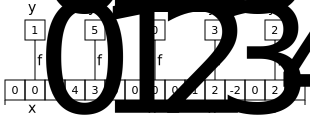
\includegraphics[width=\textwidth]{pattern-map.png}
	\caption{
		Visualization of the map pattern.
		3-vectors are mapped to their lengths.
		Because the two data types have different sizes the operation is not performed in-place.
	}
	\label{fig:map}
\end{figure*}
If $t_x$ and $t_y$ have the same size map can be performed in-place, requiring only $O(M)$ extra memory.
If $x$ needs to be re-used or if $t_x$ and $t_y$ have different sizes a new array needs to be allocated for $y$.
Under the assumption that $f$ takes a constant amount of time to compute map is embarrassingly parallel.
\subsection{Reduce}
\label{reduce}
The \textit{reduce} pattern condenses all values of $x$ into a single value $y$.
In order for this pattern to work $y$ must have the same data type as $x_i$ and
there must be an associative operator $\oplus: (t_x, t_x) \rightarrow t_x$ that carries out the reduction.
A simple way to implement the reduce pattern is to again divide $x$ into segments and assign each segment to a different SP.
Then each segment is reduced with $\oplus$ to a single value $y_n$.
The values $y_n$ can then in turn be iteratively reduced:
first $\frac{N}{2}$ SPs reduce the $y_n$ to just $\frac{N}{2}$ values while $\frac{N}{2}$ SPs are idling,
then $\frac{N}{4}$ SPs reduce the $\frac{N}{2}$ from the previous iteration to $\frac{N}{4}$ new values while $\frac{3N}{4}$ SPs are idling,
and so on until the $y_n$ have been reduced to a single value.
An example is shown in figure \ref{fig:reduce}.
\begin{figure*}
	\centering
	\includegraphics[width=\textwidth]{pattern-reduce.png}
	\caption{
		Visualization of the reduce pattern.
		Integers are summed up to a single value.
		In this example four streaming processors/CPU cores are used.
	}
	\label{fig:reduce}
\end{figure*}

The implementation described above is embarrassingly parallel if $N >> M$.
In this case the work of reducing the individual segments into $y_n$ is dominant
and the SPs will only spend a small amount of time idling at the end.
The described implementation would also only require $O(M)$ extra memory and have a runtime of $O(N)$.

As an example, let us consider calculating the sum of an array of integers.
With the reduce pattern each SP would sum up part of the array to create partial sums.
The partial sums are then iteratively added up to the total sum of the array.

In regards to sums there is an important caveat though:
most operations on floating point numbers, particularly additions, are \textbf{not} associative.
Because floating point numbers only have a limited precision their operations are subject to rounding errors.
As such, applying the parallel reduce pattern to an array of floating point numbers will usually yield a slightly different result
compared to a sequential execution.
The techniques for minimizing the floating point error are the same for sequential and parallel execution though,
and they are as such beyond the scope of this document.
\subsection{Filter}
The \textit{filter} pattern is - as the name implies - used to filter an array based on some criterion:
elements that fulfill the criterion are kept while elements that don't are discarded.
This can be achieved by defining a function $f: t_x \rightarrow \textbf{bool}$ and keeping only those elements $x_i$
where $f(x_i)$ is evaluated to \textit{true}.
As with map the filter pattern for a single element $x_n$ can be evaluated independently from all other elements.
As such, the same simple strategy of separating $x$ into segments and working on each segment in parallel can be used.
However, because the array produced by the filter pattern is of a different size
compared to the input array the filter pattern cannot be performed in-place.
The elements filtered by each SP need to be copied to a new array and possibly copied again at the end to form a contiguous array.
An example is shown in figure \ref{fig:filter}.
\begin{figure*}
	\centering
	\includegraphics[width=\textwidth]{pattern-filter.png}
	\caption{
		Visualization of the filter pattern.
		Only integers smaller than 4 are accepted.
		The operation is not in-place.
	}
	\label{fig:filter}
\end{figure*}

The implementation described above is embarrassingly parallel if $N >> M$
since in this case the time needed for filtering the segments is dominant.
Due to having to create a new array the described implementation is $O(N)$ both in terms of extra memory and runtime.
